\chapter{Speech to Text}
\ifpdf
    \graphicspath{{Chapter3/Chapter3Figs/PNG/}{Chapter3/Chapter3Figs/PDF/}{Chapter3/Chapter3Figs/}}
\else
    \graphicspath{{Chapter3/Chapter3Figs/EPS/}{Chapter3/Chapter3Figs/}}
\fi

\textit{Nội dung chương 3 sẽ giới thiệu tổng quan về bài toán Speech to Text, mô hình hoạt động, các ứng dụng của Speech to Text, các vấn đề cần giải quyết của module Speech to Text trong một hệ thống trợ lý ảo và cách giải quyết các vấn đề đó. Chương 3 cũng sẽ giới thiệu về chức năng, cách cài đặt, cách sử dụng cũng như các ưu nhược điểm của các thư viện pocketsphinx và Google Speech to Text.}

\section{Tổng quan}

Speech to Text, hay Speech Recognition là một lĩnh vực trong khoa học máy tính, trong đó nghiên cứu và phát triển các phương pháp và công nghệ để máy tính có thể nhận biết và chuyển đổi ngôn ngữ nói sang dạng văn bản. Speech recognition là một bài toán khó dành cho các nhà khoa học, vì tiếng nói luôn thay đổi theo thời gian và có sự khác biệt giữa tiếng nói của những người khác nhau, tốc độ nói, ngữ cảnh và môi trường khác nhau.

Những hệ thống speech recognition đầu tiên trên thế giới có khả năng nhận biết rất hạn chế: số lượng từ vựng mà chúng có thể nhận biết chỉ ở mức vài chục, và chỉ có thể nhận biết chính xác nếu người dùng nói một cách rất rõ ràng. Ngày nay, với sự phát triển bùng nổ của deep learning và big data, các công nghệ speech recognition cũng đã phát triển rất nhanh về số lượng từ vựng và độ chính xác. Các hệ thống speech recognition hiện đại nhất có thể nhận biết được hàng chục nghìn, thậm chí là hàng trăm nghìn từ khác nhau, và độ lỗi khi nhận biết đã giảm đến gần mức nhận biết của con người. Ngày càng nhiều công ty công nghệ đã tham gia vào cuộc đua về speech recognition, có thể kể đến Google, Microsoft, IBM, Baidu, Apple, Amazon,...

\section{Mô hình hoạt động}

Hiện nay có rất nhiều kỹ thuật khác nhau để phát triển speech recognition. Tuy nhiên có thể nhận thấy một điểm chung của đa phần các kỹ thuật này là các mô hình thống kê, trong đó nổi bật là Hidden Markov Model (HMM).

Khi huấn luyện, các câu nói trong tập dữ liệu sẽ thường được chia thành các thành phần âm (phonemes), tín hiệu âm thanh đầu vào thường sẽ được chia thành những đoạn ngắn, đưa qua các bước tiền xử lý như FFT hoặc MFCC để trích xuất đặc trưng. Hệ thống speech recognition sẽ sử dụng HMM để tìm sự liên hệ giữa các phonemes và các đặc trưng của tín hiệu âm thanh. Khi đó, khi một đoạn âm thanh mới được đưa vào, HMM sẽ trả về những chuỗi âm có thể tương ứng với đoạn âm thanh đó. Mô hình này được gọi là acoustic model.

Bên cạnh acoustic model, người ta cũng sẽ tạo ra các language model. Language model thường sẽ gồm:

\begin{itemize}
    \item Danh sách các từ (gọi là từ điển). Hệ thống sẽ nhận biết được những từ nằm trong từ điển này.
    \item Cấu trúc âm của các từ trong từ điển, ví dụ như từ "stuff" gồm 3 âm: "st", "uh" và "ff".
    \item Mối quan hệ giữa các từ trong từ điển (từ nào thường đứng cạnh từ nào).
\end{itemize}

Language model sẽ nhận các chuỗi âm output từ acoustic model, tìm cách ghép các chuỗi âm này thành các chuỗi từ có trong từ điển, và tìm cách ghép các chuỗi từ này thành câu.

\begin{figure}[h]
    \centering
    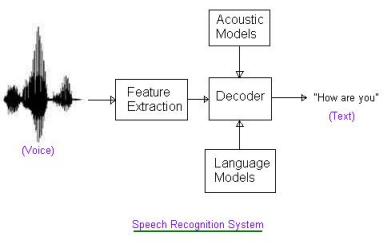
\includegraphics[scale=1]{SRSystem}
    \caption{Cấu trúc một hệ thống speech recognition đơn giản}
    \label{fig:c3_SRSystem}
\end{figure}

Ngoài HMM, nhiều mô hình khác cũng đã được các nhà phát triền speech recognition sử dụng để thay thế hoặc hỗ trợ cho HMM như Gaussian Mixture Model, Deep Neural Networks, Recurrent Neural Networks, Finite-State Transducers...

\section{Ứng dụng}

\begin{itemize}
    \item Chuyển hướng cuộc gọi tự động, quay số bằng giọng nói, tìm kiếm bằng giọng nói.
    \item Dùng trong việc ra lệnh bằng giọng nói trên các máy bay quân sự.
    \item Dùng trong các ứng dụng dạy học ngoại ngữ.
    \item Phụ đề tự động trong các video.
    \item Điều khiển robot bằng giọng nói.
    \item Hỗ trợ người khuyết tật.
    \item Phiên dịch tự động.
    \item ...
\end{itemize}

\section{Các vấn đề cần giải quyết}

Speech to Text luôn đóng vai trò là một trong những phần quan trọng nhất trong một ứng dụng trợ lý ảo. Trong một hệ thống trợ lý ảo điển hình, sẽ có hai vấn đề lớn về speech recognition: dò tìm keyword và chuyển đổi lệnh của người dùng thành văn bản.

\subsection{Dò tìm keyword}

Mỗi hệ thống trợ lý ảo sẽ được xác định trước một keyword, keyword này sẽ được dùng để kích hoạt trợ lý ảo. Mỗi khi người dùng gọi keyword này, ứng dụng sẽ chuyển sang trạng thái thu âm để ghi nhận lệnh từ phía người dùng. Keyword này thường là một từ hoặc cụm từ ngắn, dễ phát âm và dễ nhận biết, và thường chứa tên của ứng dụng, ví dụ như của Google Assistant là "OK Google", của Siri là "Hey Siri",...

\subsubsection{Yêu cầu}

Thứ nhất, chức năng dò tìm keyword của hệ thống phải hoạt động liên tục trong suốt quá trình ứng dụng chạy, do hệ thống phải có phản ứng ngay lập tức khi người dùng gọi keyword. Nếu chức năng này bị gián đoạn, hệ thống sẽ dễ bỏ lỡ mất keyword. Do đó, phần nhận biết tiếng nói trong chức năng này nên hoạt động offline, để tránh những gián đoạn trên đường mạng.

Thứ hai, tốc độ nhận biết keyword phải rất nhanh. Hệ thống sẽ liên tục thu âm từ microphone thành các frame âm thanh để xử lý liên tục trong thời gian thực, và phải liên tục kiểm tra các đoạn âm thanh liên tiếp nhau xem có chứa keyword hay không. Khi phát hiện ra một đoạn âm thanh thu được có chứa keyword, hệ thống phải ngay lập tức phản hồi lại cho người dùng và chuyển sang trạng thái thu âm lệnh của người dùng. Nếu tốc độ nhận biết keyword chậm, việc chuyển trạng thái sang thu âm sẽ bị trễ, và lệnh của người dùng khi thu vào có thể sẽ không đầy đủ, dẫn tới phản hồi sai.

Thứ ba, độ chính xác của việc nhận biết keyword phải đạt mức tương đối cao. Do từ khóa được chọn là một từ dễ đọc và dễ nhận biết nên độ chính xác của chức năng này không cần phải quá cao. Ngoài ra việc đặt ngưỡng nhận biết ở mức không quá cao sẽ làm hạn chế tối đa số lượng false negatives (trường hợp người dùng gọi keyword nhưng ứng dụng không nhận ra). Tuy nhiên điều đó sẽ làm gia tăng số lượng false positives (trường hợp người dùng không gọi keyword nhưng ứng dụng lại nhận ra), do đó cần phải tìm giải pháp để giảm số lượng false positives này.

\subsubsection{Giải pháp}

Trong hệ thống này, chúng tôi sẽ sử dụng thư viện pocketsphinx để cài đặt chức năng phát hiện keyword. Đây là một thư viện speech recognition có khả năng hoạt động offline, tốc độ xử lý nhanh, tuy nhiên độ lỗi của thư viện này là lớn hơn so với một vài thư viện khác.

Ngoài ra, ngay khi pocketsphinx nhận ra được keyword trong một đoạn âm thanh, hệ thống sẽ gửi đoạn âm thanh đó vào thư viện Google Speech to Text để kiểm tra lại một lần nữa. Hai bước kiểm tra qua hai model khác nhau sẽ giúp hệ thống hạn chế được số lượng false positives.

\subsection{Chuyển đổi lệnh người dùng thành văn bản}

Sau khi phát hiện ra keyword, hệ thống sẽ được kích hoạt và bắt đầu thu âm lệnh của người dùng. Sau khi người dùng nói xong, hệ thống sẽ phải chuyển lệnh của người dùng sang dạng văn bản để có thể xử lý và hiểu được lệnh đó.

\subsubsection{Yêu cầu}

Phần chức năng chuyển đổi câu lệnh của người dùng thành văn bản chỉ bắt đầu hoạt động khi người dùng muốn ra lệnh, tức là sau khi người dùng gọi keyword, còn những khoảng thời gian khác, chức năng này sẽ nằm ở trạng thái chờ. Việc thu âm lệnh người dùng chỉ ngừng lại khi người dùng ngừng ra lệnh. Nếu hệ thống ngừng thu âm quá sớm, lệnh của người dùng thu vào sẽ bị thiếu và không chính xác. Nếu hệ thống ngừng thu âm quá muộn sẽ tạo ra độ trễ lớn từ lúc người dùng ra lệnh đến lúc ứng dụng phản hồi, và có thể tạp âm sau khi người dùng nói xong sẽ lọt vào phần speech recognition khiến kết quả nhận biết bị sai lệch.

Ngoài ra, độ chính xác của việc chuyển lệnh của người dùng về văn bản phải đạt mức rất cao, để đảm bảo hệ thống có thể hiểu đúng được ý định của người dùng.

\subsubsection{Giải pháp}

Trong hệ thống trợ lý ảo này, module chuyển đổi lệnh người dùng thành văn bản được cài đặt sử dụng thư viện Google Speech to Text. Đây là công cụ nhận biết tiếng nói của Google được đánh giá rất cao về độ chính xác, nhờ đó hệ thống sẽ đảm bảo hiểu đúng được hầu hết các lệnh của người dùng.

Để việc thu âm có thể ngừng đúng lúc, trong hệ thống sẽ có một giá trị thời gian $T$ và một ngưỡng cường độ $D$. Khi âm thanh thu được từ microphone có cường độ nằm dưới mức $D$ trong một khoảng thời gian $T$ liên tục thì hệ thống sẽ xem như người dùng đã kết thúc việc ra lệnh và dừng trạng thái thu âm để bắt đầu xử lý đoạn âm thanh đã thu được.

\section{Thư viện pocketsphinx}

\subsection{Tổng quan}

Pocketsphinx là một thư viện speech recognition mã nguồn mở được phát triển bởi Viện Công nghệ Ngôn Ngữ, thuộc trường Đại học Carnegie Mellon (Mỹ). Pocketsphinx là phiên bản tối ưu của CMU Sphinx-II, cũng là một hệ thống nhận dạng tiếng nói khá nổi tiếng của ĐH Carnegie Mellon. Nhóm nghiên cứu này đã tối ưu hóa pocketsphinx rất nhiều về bộ nhớ và thuật toán, nhằm có thể tạo ra một thư viện nhận dạng tiếng nói liên tục có khả năng đưa vào các thiết bị cầm tay.

Hệ thống của pocketsphinx chủ yếu dựa trên những mô hình phổ biến của speech recognition như Gaussian Mixture Model và thuật toán Viterbi trên Hidden Markov Model, kết hợp với nhiều thuật toán hỗ trợ khác\cite{huggins2006pocketsphinx}.

Pocketsphinx được đánh giá cao nhờ vào khả năng hoạt động offline và tốc độ xử lý khá nhanh. Ngoài ra, pocketsphinx có khả năng xử lý real-time liên tục trên stream âm thanh (thay vì phải hoàn tất việc thu âm và xử lý trên file âm thanh thu được).

\subsection{Cách cài đặt}
\begin{itemize}
\item Windows, Mac OS, Linux: \lstinline[language=bash]{pip install pocketsphinx}
\end{itemize}
\subsection{Cách sử dụng}
\begin{itemize}
\item Trước hết, để khởi tạo thư viện Pocketsphinx ta cần thực hiện 3 bước:
\begin{itemize}
\item Bước 1: Khởi tạo đối tượng config.
\item Bước 2: Khởi tạo các tham số cho đối tượng config. Trong đó:
\begin{itemize}
\item \lstinline{-hmm}: đường dẫn đến thư mục chứa Hidden Markov model của thư viện. Đối với ngôn ngữ Anh, thư mục này có tên là "en-us" và nằm tại thư mục mà thư viện được cài.
\item \lstinline{-dict}: đường dẫn đến tập tin từ điển của thư viện. Tập tin này thường có tên là "cmudict-en-us.dict" đối với ngôn ngữ Anh.
\item \lstinline{-keyphrase}: là keyword mà bạn muốn pocketsphinx theo dõi.
\item \lstinline{-kws_threshold}: là ngưỡng dùng để xác định độ nhạy của pocketsphinx. Ngưỡng này càng thấp thì pocketsphinx càng nhạy, nghĩa là khả năng False Positive khi dò tìm keyword cũng sẽ tăng. Ngược lại, ngưỡng này càng cao thì pocketsphinx càng kém nhạy, khả năng bỏ lỡ keyword (False Negative) sẽ tăng lên.
\end{itemize}
\item Bước 3: Khởi tạo pocketsphinx bằng đối tượng config.
\end{itemize}

Đoạn mã mô phỏng cách khởi tạo thư viện Pocketsphinx
\begin{lstlisting}
from pocketsphinx import *

#step 1
config = Decoder.default_config()

#step 2
config.set_string('-hmm', "path to hmm model")
config.set_string('-dict', "path to dict")
config.set_string('-keyphrase', "keyword")
config.set_float('-kws_threshold', threshold)

#step 3
self.decoder = Decoder(config)
\end{lstlisting}

\item Sau khi khởi tạo, ta sẽ bắt đầu dò keyword bằng cách gọi hàm \lstinline{start_utt()}. Lần lượt đọc dữ liệu âm thanh input và xử lý bằng hàm \lstinline{process_raw(data)}. Ta kiểm tra kết quả trả về của hàm \lstinline{hyp()}, nếu kết quả khác \lstinline{None} nghĩa là đã dò thấy keyword.

Đoạn mã mô phỏng cách sử dụng pocketsphinx để dò keyword
\begin{lstlisting}
self.decoder.start_utt()
while True:
	data = readInputData()
	self.decoder.process_raw(data, False, False)
			if self.decoder.hyp() != None:
				# Keyword detected
				self.decoder.end_utt()
				self.decoder.start_utt()
\end{lstlisting}
\end{itemize}
\subsection{Các ưu, nhược điểm}

\begin{itemize}
    \item \textbf{Ưu điểm:} Hỗ trợ xử lý offline, xử lý real-time liên tục, hỗ trợ chức năng dò tìm keyword.
    \item \textbf{Nhược điểm:} Độ chính xác khá kém. Độ lỗi word error rate khi thử nghiệm của pocketsphinx lên đến 13.95\%\cite{huggins2006pocketsphinx}.
\end{itemize}

\subsection{Ứng dụng}

Trong hệ thống trợ lý ảo của khóa luận này, pocketsphinx sẽ được sử dụng trong module WakeUp. Pocketsphinx sẽ giúp phát hiện ra khi người dùng gọi wake-up word, qua đó kích hoạt hệ thống.

\section{Thư viện Google Speech To Text}

\subsection{Tổng quan}

Google Speech Recognition là hệ thống nhận biết tiếng nói do Google nghiên cứu và phát triển. Hệ thống này đã được Google tích hợp vào trợ lý ảo Google Assistant trên các thiết bị Android và loa thông minh Google Home, và cũng đã được đưa vào ứng dụng tìm kiếm Google Search. Google cũng đã đưa ra Google Speech API cho phép các lập trình viên sử dụng hệ thống speech recognition này vào các ứng dụng của họ. Google Speech to Text là một thư viện trên Python có khả năng nhận biết tiếng nói nhờ vào việc gọi đến Google Speech API.

Trong quá trình phát triển, các nhà nghiên cứu của Google đã sử dụng nhiều kỹ thuật khác nhau cho Google Speech Recognition, từ những kỹ thuật cổ điển như Gaussian Mixture Model, đến những kỹ thuật hiện đại hơn như Deep Neural Networks hay Long Short-term Memory Recurrent Neural Networks (LSTM RNNs)\cite{beaufays}.

Nhờ sự thay đổi và tiến bộ liên tục, Google Speech Recognition được đánh giá rất cao về độ chính xác của mình. Tại Google I/O 2017, Google đã công bố độ chính xác của công nghệ nhận biết tiếng nói này đã đạt độ lỗi word error rate là 4.9\%\cite{protalinski}, tức là độ chính xác lên đến hơn 95\%.

\subsection{Cách cài đặt}
\begin{itemize}
\item Windows, Mac OS, Linux: \lstinline[language=bash]{pip install SpeechRecognition}
\end{itemize}

\subsection{Cách sử dụng}
\begin{itemize}
\item Thư viện Google Speech to Text sử dụng hết sức đơn giản gồm 2 bước
\begin{itemize}
\item Bước 1: Import module \lstinline{speech_recognition} và lớp \lstinline{AudioData}.
\item Bước 2: Gọi hàm \lstinline{sr.Recognizer().recognize_google} để thu được văn bản kết quả. Chú ý hàm này không thể xử lý trực tiếp với dữ liệu âm thanh thô mà phải được bao bởi lớp AudioData với các tham số:
\begin{itemize}
\item \lstinline{audio}: dữ liêu âm thanh thô
\item \lstinline{sample_rate}: tần số lấy mẫu của âm thanh.
\item \lstinline{sample_width}: số byte dùng để biểu diễn mỗi mẫu của âm thanh.
\end{itemize}
\end{itemize}
\end{itemize}

Đoạn mã mô phỏng cách sử dụng thư viện Google Speech to Text
\begin{lstlisting}
#step 1
import speech_recognition as sr
from speech_recognition import AudioData

#step 2
text = sr.Recognizer().recognize_google(AudioData(audio, sample_rate, sample_width))
\end{lstlisting}

\subsection{Các ưu, nhược điểm}

\begin{itemize}
    \item \textbf{Ưu điểm:} Độ chính xác rất cao.
    \item \textbf{Nhược điểm:} Yêu cầu internet để hoạt động, không xử lý real-time trên stream âm thanh được mà phải gửi toàn bộ file âm thanh.
\end{itemize}

\subsection{Ứng dụng}

Trong hệ thống này, thư viện Google Speech to Text được dùng trong module SpeechToText. Module này sẽ đóng vai trò chuyển đổi những câu lệnh của người dùng từ dạng âm thanh sang dạng văn bản.
